\begin{savequote}[75mm]
OMG... Is that a neuron??
\qauthor{An Excited Grad Student}
\end{savequote}

% Ephys:
% (Jun et al., 2017 (neuropixels); 
% Siegle et al., 2019 (hierarhcy, Nature)
% Stringer et al., 2019a -- spontaneous bebaviors, Science

% ca imaging: 
% (Sofroniew et al., 2016; -- meoscope, elife
% Stringer et al., 2019b --high-dim geometry, Nature
% Weisenburger et al., 2019). --- alipasha, Cell

\chapter{Engineering systems for optical imaging in rats}
% INTRO
\newthought{Large-scale recordings} of hundreds and even thousands of neurons are becoming increasingly standard using electrophysiology \cite{Steinmetz2019DistributedBehaviour, REFREF} and optical imaging \cite{Stringer2019High-dimensionalCortex, REFREF}. With rapid advancements in genetic tools, hardware design, and computational power, we are in an unprecedented and exciting time to be studying neural circuits and behavior. For measuring neural populations in an awake animal, there are two main classes of methods, imaging and electrophysiology. Both are extremely powerful, and choosing one or the other is highly dependent on the goals of the experiment. 

Electrophysiology provides the most direct access to neural activity, as it measures voltage changes with high temporal resolution, allowing for measurements of single spikes and sub-threshold activity\cite{REFREF}. It is also amenable to tethered or even wireless systems that allow animals to move about relatively freely, thus allowing a more naturalistic setting for studying neural circuits and behavior in the lab\cite{REFREF}. However, long-term access to a given neuron and the throughput of how many neurons can be recorded simultaneously is limited by the uncertainties in single unit isolation, the capacities of electronic components, and how many channels one can physically fit and successfully record from in a small animal. 

In contrast, optical approaches allow the same cells to be tracked for long periods of time, and simultaneous recording of large populations (hundreds to thousands) in the same animal. Optical imaging of neural activity relies on genetic tools that enable fluorescent indicators to be expressed in targeted cell populations. Standard approaches rely on tracking changes in calcium activity that occur in response to voltage changes in a neuron\cite{REFREF}. As such, the measured signal is slower and not a direct readout of neural activity, as measured by electrophysiology. Instead, calcium activity is measured by way of genetically-encoded fluorescent calcium indicators (GECIs)\cite{Akerboom2012, Chen2013}, which fluoresce in response to calcium binding. In transgenic animals, these indicators can be expressed in a controlled manner, from sparse labeling\cite{REFREF} to pan-neuronal expression\cite{REFREF}. In the absence of a transgenic animal or in combination with one that expresses a different gene of interest, one can also use viral vectors, such as an adeno-associated virus (AAV) or lentivirus\cite{REFREF} for robust delivery of the GCaMP construct, and expression of the indicator remains robust and stable over at least several months\cite{REFREF}.

Physical access to deep or lateral parts of the brain is limited with optical methods, which typically rely on imaging the brain from directly above the animal's head. Many optical systems are bulky, making it quite difficult to record from freely moving animals. While electrodes can be inserted deep and at any angle into the brain, optical access to deeper brain structures sometimes requires removing superficial layers\cite{REFREF}, or using mirrors to direct the light path in clever ways while keeping the collection system above the animal\cite{Andermann2013}. Head-mounted optical systems allow for cellular resolution imaging in freely moving animals\cite{miniscope, Helmchen2001, Sawinski2009, 3photonmini}, and high-photon-count imaging (\textit{e.g.}, >3 photon\cite{REFREF}) improve optical access to deeper brain structure

However, the gap between the two methods continues to get smaller, as technological advancements offer improvements to the challenges each face. There continue to be major technical advances in electrophysiological approaches, such as high-density electrode arrays\cite{REFREF} and computational methods for processing high channel count data and verifying chronic access to specific cells\cite{REFREF}. For imaging, each generation of calcium indicators has proved increasingly more powerful, \textit{e.g.}, higher signal-to-noise (SNR), multi-color alternatives, and higher temporal resolution \cite{Akerboom2012OptimizationImaging, Chen2013UltrasensitiveActivity, REFREF}. Progress has also been made toward developing voltage-sensitive indicators\cite{REFREF, Adam Cohen, etc}, which have the potential to combine the advantages of spatial and genetic access provided by optical methods with the more direct signal and higher temporal resolution of electrophysiology. High-photon-count imaging (\textit{e.g.}, >3 photon \cite{REFREF}) improve optical access to deeper brain structure.

Today, one of the greatest advantages of optical imaging is cellular resolution access to large swaths of the brain. To be able to visualize single neurons as a population in awake animals is immensely powerful, especially in concert with sophisticated manipulation techniques, such as multi-channel optogenetics \cite{REFREF}, holographic light stimulation \cite{REFREF}, and genetically-defined targeting of specific populations of cells. In combination, these features allow one to measure and manipulate the same neurons in awake, behaving animals across large numbers of stimuli and trials over the course of weeks and months. In contrast, conventional acute single-unit microelectrode recordings are limited by the time that a single cell can be isolated (usually only one or a few hours). Even the best chronic preparations face difficulties holding isolated cells over very long time periods, and it is difficult to be absolutely confident that the same cell is isolated across days, especially given that nearby cells are often thought to have similar response properties.

%% % What has been done, and what's missing  ---------------------------
For cellular resolution imaging, most studies rely on head-fixed preparations in which that animal's head is fixed in place for clear optical access. Multi-photon imaging systems are usually table-top designs, as the equipment is quite bulky and stable imaging planes are needed for quality imaging. Miniature head-mounted two-photon microscopes offer an alternative to head-fixation during in vivo imaging \cite{Helmchen2001, Piyawattanametha2009, Sawinski2009}. Such techniques can be powerful for measuring neural activity in a wide range of naturalistic behaviors \cite{Sawinski2009}, but the technical difficulty of using these miniaturized microscopes has limited their use as a standard tool in neuroscience \cite{Kerr2012}. Furthermore, many other in vivo imaging technologies are difficult to miniaturize, preventing their use as head-mounted devices. 

Studies using head-fixed animals have access to certain experimental advantages, such as restrained movement, precise stimulus control, and longitudinal studies that can track the same neurons over long timescales. While head-fixed preparations are routinely used in flies and mice {REFREF}, rats are much harder to restrain with these protocols, given their larger size and prohibitive movement artifacts for cellular-resolution imaging. As such, most studies using head-fixed rats rely on electrophysiology. Furthermore, the lateral position of many brain areas of interest in the rat (see Introduction) makes optical access all the more challenging, and most rat imaging studies have been restricted to primary visual cortex, V1\cite{Greenberg2008, Ohki2005, Scott2018}.

Although a large body of scientific research relies on the rich behavioral repertoire of rats, it has not been possible to fully leverage recent developments in optical imaging and molecular and genetic tools, as has been done with great success in smaller animals like mice. In one heroic study, Scott \textit{et al.} developed a method for training rats to voluntarily head-fix themselves into a two-photon system, which allowed for cellular resolution imaging in awake, behaving rats \cite{Scott2013}. However, voluntary head-fixation can be difficult and time-intensive, and if successful for a given rat, still places significant limitations on how much control the experimenter can have over the time course of the study. More recently, the same group also created a transgenic rat expressing GCaMP in all neurons, and demonstrated the feasibility of recording population dynamics in awake, freely moving rats, albeit without cellular resolution\cite{Scott2018ImagingMacroscope}. 

% FIGURE 2.1 Rat visual areas
\begin{figure}[t!]
    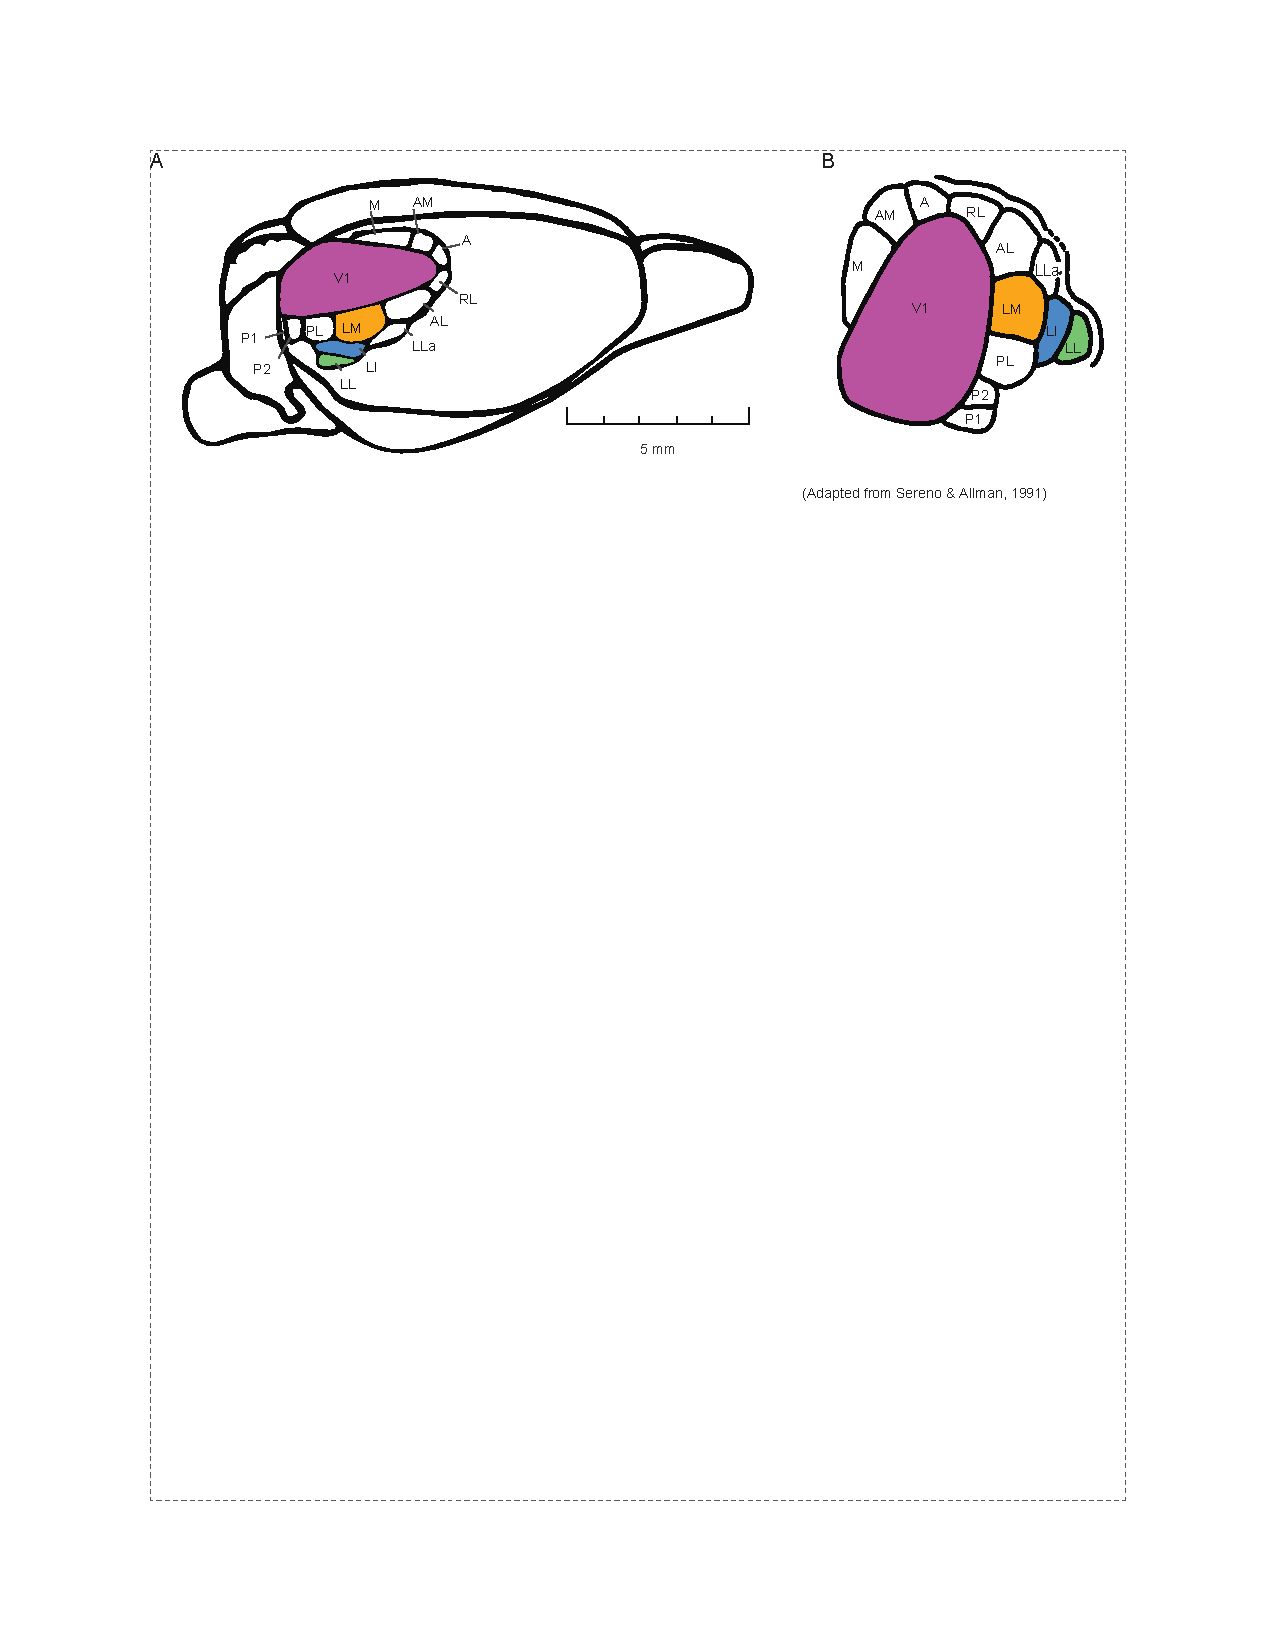
\includegraphics[width=\textwidth]{figures/chapter_2/fig_2-1_rat_visual_areas/fig_2-1_rat_visual_areas.pdf}
    \vspace{.1in}
    \caption[Visual areas in the rat]{Visual areas in the rat. \textbf{A.} Lateral view of visually responsive areas identified by electrophysiological mapping of retinotopic preference. \textbf{B.} Flattened representation of lateral visual areas, with targets of the present study, areas V1, LM, and LI, highlighted in color. 
    \label{fig:rat_visual_areas}}
\end{figure}

Almost all of our knowledge about rat visual cortex comes from electrophysiology studies. To date, the only area of visual cortex to be imaged from in rats is primary visual cortex, or V1, from intrinsic signal \cite{Gias2004} to single-photon \cite{Scott2018ImagingMacroscope} and two-photon \cite{Ohki2005, Greenberg2008} imaging. However, rat visual cortex contains several areas, the largest of which is striate or primary visual cortex, or V1, with additional extrastriate areas surround V1 \cite{Espinoza1983RetinotopicRat, Sereno1991} (Figure~\ref{fig:rat_visual_areas}). In rats, areas V1, LM, LI, and LL lie along the medial-to-lateral axis at the posterior edge of the brain, extending well beyond the lateral bone ridge. These visual areas have gained significant interest within the last ten years, as neurons in these areas, as measured by electrophysiology, appear to have several functional similarities to those characterized along the ventral stream of the primate brain (see Introduction). 

With genetic tools becoming increasingly available in rats, there is immense potential for a head-fixed system in which many of these tools can be fully leveraged has immense potential. We developed a method for cellular-resolution imaging of large FOVs in awake, head-fixed rats with the ultimate goal of chronic cellular resolution access to the visual cortex of rats. 

\section{Procedures for optical access and long-term viability} 
% %%%%%%%%%%%%%%%%%%%%%%%%%%%%%%%%%%%%%%%%%%%%%%%%%%%%%%%%%%%%%%%%
% Surgery + implant
% %%%%%%%%%%%%%%%%%%%%%%%%%%%%%%%%%%%%%%%%%%%%%%%%%%%%%%%%%%%%%%%%
% fig:experimental_pipeline
% fig:surgery_steps
% fig:headplate_schematic
% fig:retino_mapping
% fig:2p_schematic
%fig:multiday_imaging

% Figure: Experimental workflow
\begin{figure}[t!]
    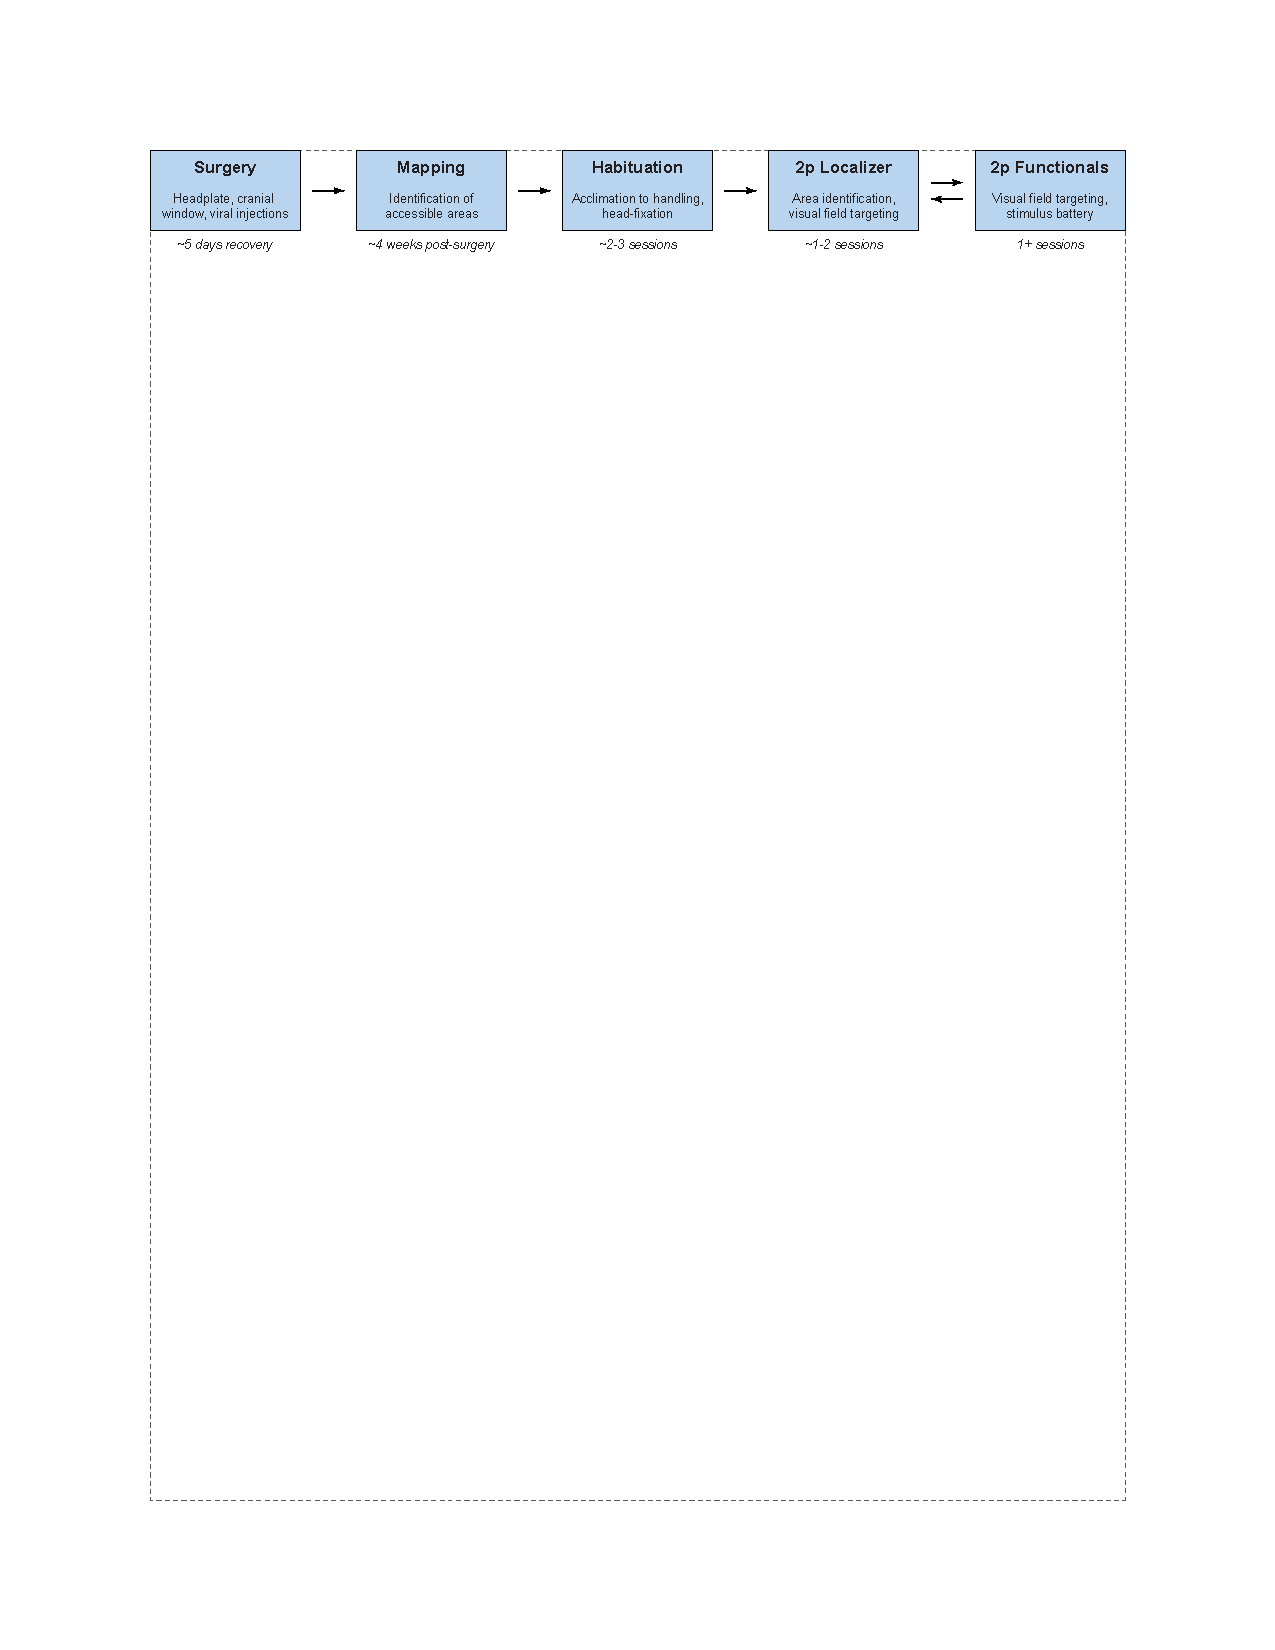
\includegraphics[width=\textwidth]{figures/chapter_2/fig_2-2_experiment_workflow/fig_2-2_experiment_workflow.pdf}
    \vspace{.1in}
    \caption[Experiment workflow]{Experiment workflow. \textit{Surgery:} Animals first undergo chronic implant and cranial window surgery. Viral delivery of the calcium indicator is done during this surgery, as ~4 weeks are needed for expression to come online throughout the window. \textit{Mapping:} Once most of the window exhibits fluorescence, the mapping procedure identifies which visual areas are identifiable and accessible within the extent of the window. Viable cranial windows must meet several criteria for animals to continue through to the next stage: sufficient expression, identifiable visual areas, and any of the three areas of interest (V1, LM, or LI/LL). \textit{Habituation:} These animals are then habituated over several days in preparation for two-photon imaging. After habituation, candidate imaging sites, or fields-of-view (FOVs), are selected for two-photon characterization. \textit{Localizer:} Candidate FOVs are then mapped for a) validating visual area assignment via retinotopic preference and gradient (see Methods), and b) targeting stimulus locations in the visual field based on the receptive field positions of the cells that are available in the FOV. \textit{Functionals:} Vetted FOVs are characterized with a battery of visual stimuli. Localizer runs are repeated during functional sessions, as well. 
    \label{fig:experiment_workflow}}
\end{figure}

Optical imaging approaches allow the same field-of-view (FOV), and with multiphoton imaging, the same cells, to be imaged across multiple sessions. Our approach aimed to combine head-fixation in awake rats, optical access to multiple brain areas, and precise re-positioning for long-term studies of chronically implanted animals. Several major challenges we needed to address were:  1) implant stability against the significant mechanical forces that awake rats are able to apply, 2) motion artefacts due to large displacements in moving rats, and 3) accessibility of large FOVs over the extreme, lateral edge of the rat skull.

% Habituation + shaping
For many behaviors of interest, it is not possible to use sedatives or other anesthetics during neural recording. This is particularly true for paradigms that rely on animals performing a task or engaging in a behavior. However, not only is it difficult to acquire quality cellular resolution recordings in struggling animals, but moreover, stress has been shown to negatively impact learning rates, as well\cite{REFREF}. Thus, it was critical to establish an experimental workflow that led to a visibly calm rat, even while head-fixed for long periods of time. We developed an extensive pipeline of surgical and experimental procedures for large-scale visual characterizations in awake, head-fixed rats (Figure\ref{fig:experiment_workflow}). Rats are much larger than mice, so a key challenge was to prevent awake rats from ripping themselves out of their implants and keeping the FOV stable enough for cellular resolution imaging. 

% window surgery --------------------------------------
%\subsection{Cranial windows for chronic imaging in awake rats}
Since chronic cranial windows are almost routine procedures in mice, we first adapted a mouse surgical protocol\cite{Goldey2014} and optimized it for rats, with a focus on strong implant adhesion and long-term viability, even against the significant forces that awake rats can apply (see Methods, REFREF). For calcium imaging, we relied on viral expression of GCaMP\cite{REFREF} across an area of cortex covering about 4-6mm. A region of this size was large enough to contain multiple visual areas in the rat, based on known cortical extents of extrastriate areas (see Figure\ref{fig:rat_visual_areas}). Since the transgenic GCaMP rat \cite{Scott2018ImagingMacroscope} had not been developed yet, it was important to calibrate the correct volume, titre, and injection method for consistent, widespread expression of the virus throughout the window (see Methods). Finally, since it is not possible to image through a thinned skull or a dura, as it is in mice, we also optimized methods for successful durotomies in the rat (Figure\ref{fig:surgery_steps}). 

% Figure: Cranial window + implant
\begin{figure}[t!]
    \includegraphics[width=\textwidth]{figures/chapter_2/fig_2-3_surgery_steps/fig_2-3_surgery_steps.pdf}
    \vspace{.1in}
    \caption[Chronic cranial window]{Implant of chronic cranial windows for GCaMP imaging. \textbf{A.} Exposed cortical surface and craniotomy during a microinjection of AAV-GCaMP. Blue, dye used to visualize spread (see Methods) \textbf{B.} Bright-field view of a cranial window. \textbf{C.} Fluorescent view of GCaMP expression in a cranial window.
    \label{fig:surgery_steps}}
\end{figure}

There were several possible points of attrition before a rat became viable for imaging. In our hands, viral expression was best starting at ~4 weeks post-injection. We tried various combinations of surgical steps to optimize this time-window --- for example, starting with large viral injections through a burr hole near the site of the cranial window, then waiting four weeks before exposing the cortical surface with a craniotomy-durotomy procedure and placing the coverslip window. However, for long-term window viability and high-quality imaging, we found the most reliable approach was to combine the implant surgery and the cranial window with viral injections as close in time as possible, preferably in the same surgery. When splitting the surgical steps, waiting too long (\textit{i.e.}, a week or more) compromised the structure of the skull bone, making window placement unstable and window "clouding" (growth of tissue or an inflammatory response within the cranial window that precludes imaging) much more likely. 

% Headplate assembly
In order to access lateral visual areas while keeping the rat’s head and body in a relatively natural resting position, our approach was to tilt the imaging plane relative to the animal’s head. This meant implanting the headplate at an angle that matched that of the objective. 

% Figure: Headplate and holding the rat
\begin{figure}
    \includegraphics[width=\textwidth]{figures/chapter_2/fig_2-4_headplate_schematic/fig_2-4_headplate_schematic.pdf}
    \vspace{.1in}
    \caption[Headplate design and assembly]{Headplate design and assembly. \textbf{A.} Schematic showing the assembly for head-fixing the animal. A thick, custom-cut steel post is affixed to the platform (modular design for both habituation setups and imaging setups). An angled bracket, custom-cut to match the desired angle of the objective, contains 3 grooves that hold spherical ceramic balls (close-up, \textit{right}), which mate with the titanium headplate. \textbf{B.} Schematic of a rat skull with a custom titanium headplate positioned over the approximate location targeted for lateral extrastriate areas in the rat. Circle and inset indicate the position of the optical window implanted over these areas. A photograph of the cortical surface accessible for imaging beneath the 5-mm diameter optical window is shown to the right for illustration. 
    \label{fig:headplate_schematic}}
\end{figure}

We leveraged the high precision afforded by kinematic mounts to design custom titanium headplates that could be mounted at steep angles while preserving the capacity for precise re-positioning (Figure\ref{fig:headplate_schematic}). The headplates contained three semi-spherical grooves that mated with stainless steel ball bearings mounted to an aluminum post on the imaging platform. The headplate mated with a steel post designed to be strong enough to hold the animal stably, while keeping the view to the stimulus monitor unobstructed on one side of the animal, and on the contralateral side, sufficiently clear for the objective. Implanted animals were stably positioned at the farthest angles tested (40-45 degrees, where 0 degrees is parallel to ground, or flat on the skull).  

% %%%%%%%%%%%%%%%%%%%%%%%%%%%%%%%%%%%%%%%%%%%%%%%%%%%%%%%%%%%%%%%%
% Identifing visual areas
% %%%%%%%%%%%%%%%%%%%%%%%%%%%%%%%%%%%%%%%%%%%%%%%%%%%%%%%%%%%%%%%%
\section{Functional identification of visual areas}
% Figure: WF retino_mapping/area segmentation
Visual areas are retinotopically arranged --- each area contains a representation of the visual field called a retinotopic map, where nearby positions in physical space are represented by nearby cells on the retina, and this spatial arrangement is preserved from one part of the visual system to the next\cite{REFREF}. Conveniently, nearby visual areas have predictable ``reflections'' of retinotopic space at area boundaries. As such, distinct visual areas can be functionally identified by these mirror reflections in the representation of the visual field. To date, though several methods have been used to image neural activity in rat cortex, from intrinsic signal\cite{Gias2004} to single-photon \cite{Scott2018ImagingMacroscope} and two-photon \cite{Ohki2005, Greenberg2008} imaging, the primary visual cortex, or V1, is the only area of visual cortex to be imaged in rats.

% WIDEFIELD --------------------------------------
\subsection{A tandem-lens macroscope for wide-field imaging}
Our first step was to optically map extrastriate areas of rat visual cortex for the first time. We needed a large field-of-view (FOV) that could capture the full extent of the window (4-5$mm$ diameter). In order to ensure robust mapping with high signal-to-noise, we also needed a sufficiently shallow depth of field for avoiding out-of-focus artefacts (\textit{i.e.}, good axial resolution). To meet these needs, we developed a tilting tandem-lens epifluorescence macroscope\cite{Ratzlaff1991} (Figure\ref{fig:retino_mapping}). 

The macroscope combined two lenses in reverse configuration with a CCD camera, all custom-mounted on a rotating plate with a translating stage --- this allowed us to both rotate the imaging plane about the animal, and gave us manual control for precise positioning with manual micromanipulators. At the start of each session, we captured a high-resolution (656x492, $9.9um$ pixels) image of the surface vasculature beneath the optical window for coregistering two-photon imaging FOVs within the extents of the window. For functional imaging, we focused below the surface to ~$500um$ using micromanipulators.

% Figure:  retino_mapping (WF)
\begin{figure}
    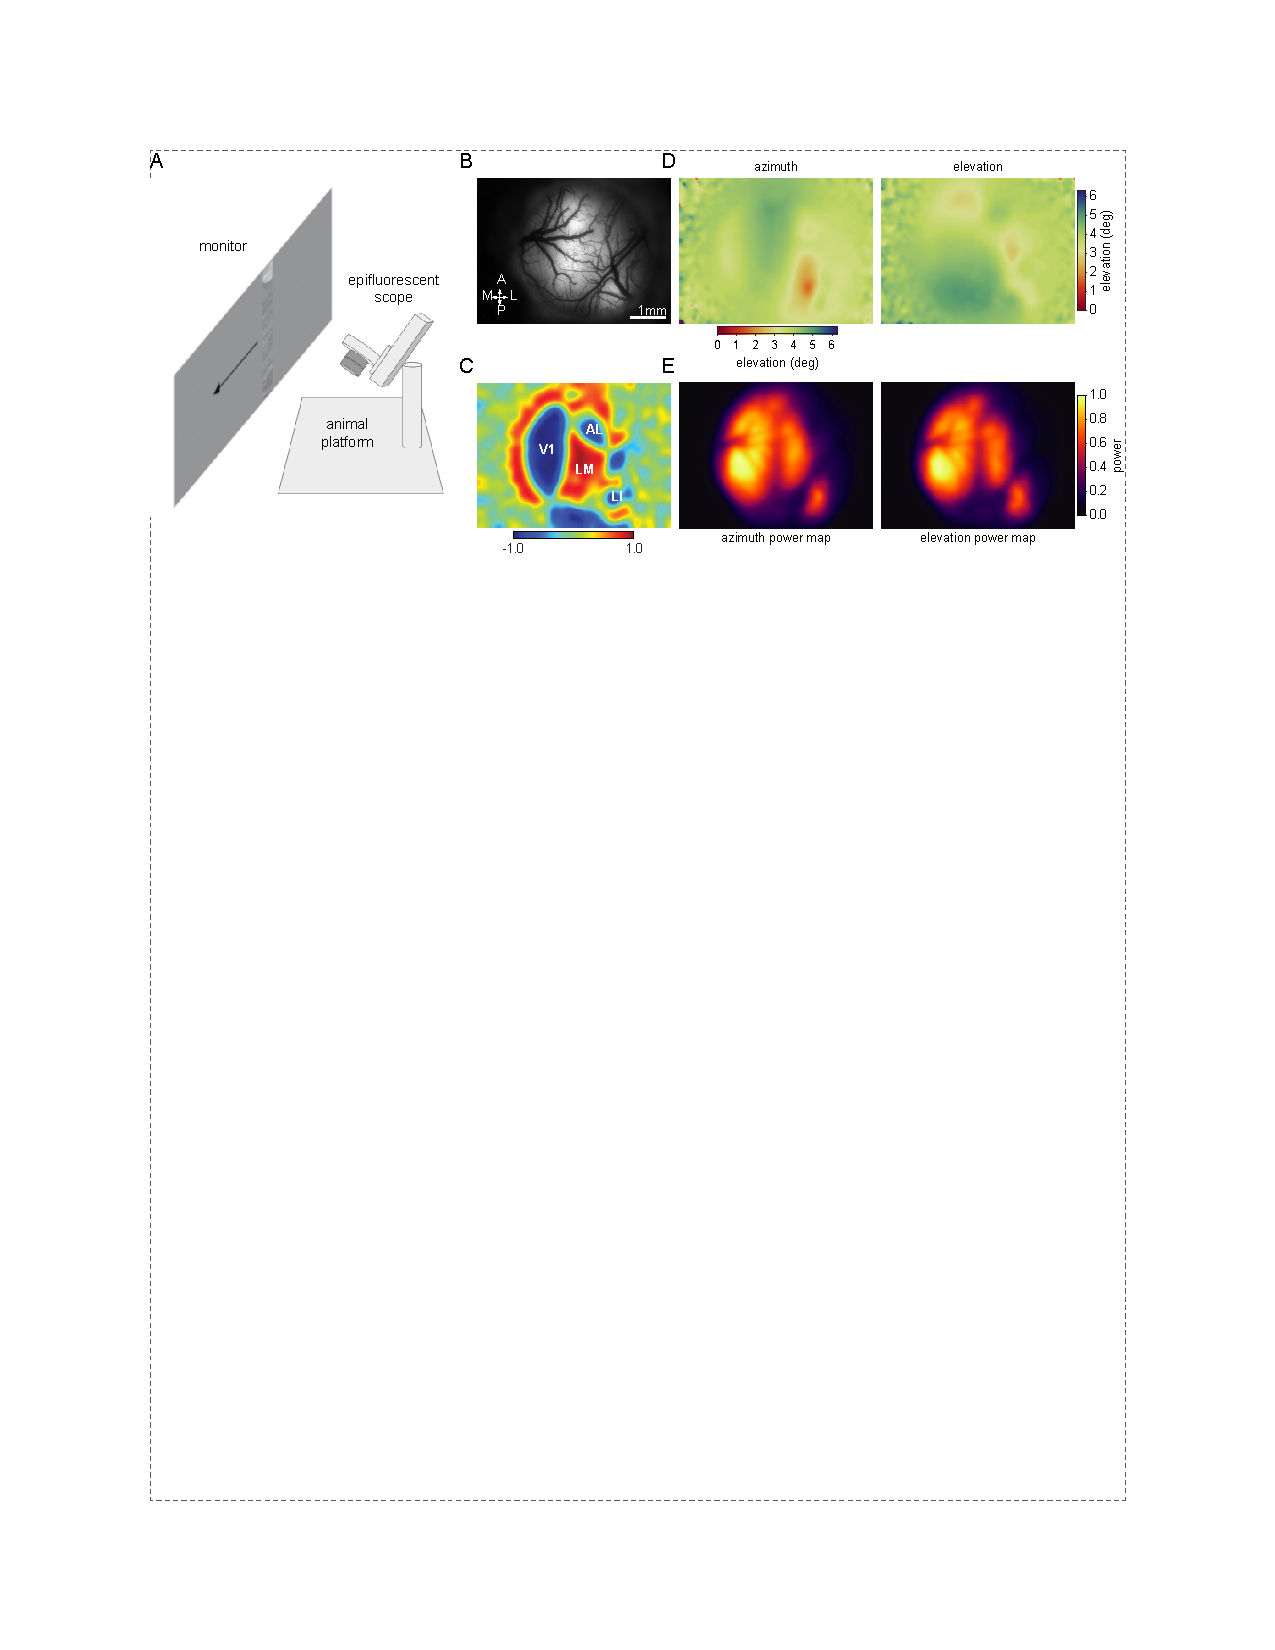
\includegraphics[width=\textwidth]{figures/chapter_2/fig_2-5_retino_mapping/fig_2-5_retino_mapping.pdf}
    \vspace{.1in}
    \caption[Wide-field mapping]{Identifying visual area boundaries. \textbf{A.} Schematic of the tandem-lens macroscope setup used for fast mapping of the entire cranial window. \textbf{B.} Widefield, epifluorescence image of the cranial window. Scale bar, 1mm. \textbf{C.} Pseudo-colored image from phase-encoded mapping of retinotopic preference along azimuth (left) and elevation (right). \textbf{D.} Sign map calculate from the gradient of the images in \textbf{C}. \textbf{E.} Normalized power for azimuth (left) and elevation (right) mapping conditions used to threshold area maps. 
    \label{fig:retino_mapping}}
\end{figure}

\subsection{Wide-field functional mapping}
For fast acquisition of retinotopic maps, we used Fourier-based calcium imaging\cite{Kalatsky2003} (Figure\ref{fig:retino_mapping}). This approach is less time-consuming (<10 minutes) than traditional event-based paradigms in which discrete positions on a monitor are stimulated one-by-one across repeated presentations to average over noisy responses, which can take many minutes or longer. In a standard Fourier-based mapping experiment, a moving bar cycles across the screen several times at at particular frequency. The position on the screen to which a given pixel best responds corresponds to a particular part of the bar's cycle, \textit{i.e.}, the phase of response at the stimulation frequency, while how strongly a pixel responds is given by the magnitude of its response at that frequency. Calculate the phase and magnitude of response for each pixel generates a 2D map of phase and magnitude. The phase map is the retinotopic map, which we use to delineate area borders base on the mirror reflections (see Figure\ref{fig:retino_mapping}), and the magnitude map can be used to filter out unresponsive pixels (and thus, remove phase values that are meaningless). 

Visual stimuli were presented using custom Python scripts (see Methods) on a large LCD monitor, which was centered in front of the left eye to span the animal's visual field left visual field (~177$^{\circ}$ of visual angle along azimuth, 67$^{\circ}$ along elevation). The mapping protocol consisted of a periodic, moving bar stimulus\cite{Kalatsky2003, Marshel2011} presented to the (left) eye contralateral to the cranial window. The bar was either a white bar drifting over a black background or an apertured bar containing a random subset of natural scene images drifting over a gray background. We did not find an clear difference between the two bar types, but qualitatively, the latter seemed quite reliable, so we primarily used the natural scene bars for the mapping sessions. The bar was presented at 0.13 Hz along the azimuth and elevation axes, for a total of 2 (downward, rightward) or 4 (downward, rightward, leftward, upward) conditions. A total of 4-5 repetitions of 10 cycles each were acquired for each direction. 

Though we tried both intrinsic imaging and calcium imaging, we found that calcium imaging in lightly anesthetized animals was the most reliable for quickly identifying the boundaries of each visual area within a given cranial window. This precluded the need for motion correction and multiple repeated session due to animal movement, as mapping was typically done prior to habituation (see Chapter REFREF, Figure\ref{fig:experiment_workflow}). Specifically, we found that with light levels of anesthesia (minimal isofluorane, 0.5-1\%, and a small dose of choloprothixene, $2mg/kg$ REFREF), such that animals woke up immediately after the isofluorane nose cone was removed, we were able to acquire strong neural signal without needing motion correction for processing the maps.

We observed smooth retinotopic maps in  V1, LM, and LI, as well as in surrounding areas, such as AL and RL across rats (Figure\ref{fig:retino_mapping}). In some animals, the cranial window spanned all three areas, but in most cases, only one or two areas were accessible with sufficient GCaMP expression for population imaging at cellular resolution (V1: REFREF rats across REFREF imaging sites, LM: REFREF rats across REFREF imaging sites, Li: REFREF rats across REFREF imaging sites, see Methods).

% Area segmentation
To segment the visual areas, we used an established method that converts the phase map into a sign map based on the gradient of the image to determine the direction reversals, which are the area boundaries\cite{Garrett2014, Zhuang2017}. We excluded any animals that had ambiguous maps (see REFREF\ref{fig:REFREF} for examples of clear and ambiguous maps). Across animals, there was some variability in which visual areas were contained within the cranial window and the patchiness of expression due to inconsistent viral spread or injections. Patchy expression presented a challenge to a fully automated segmentation approach, for example, by splitting visual areas that should be continuous, or assigning an area where viral expression and signal was quite poor. All maps were thus inspected by eye, and patch merging and smoothing parameters were manually adjusted based on visual sign consistency, size and orientation of a given visual area relative to surrounding areas (since all windows captured minimally 1-2 mirror reflections), and comparison with movies of the imaging session, which allowed direct visualization of the stimulus traveling on the cortical surface. 

% %%%%%%%%%%%%%%%%%%%%%%%%%%%%%%%%%%%%%%%%%%%%%%%%%%%%%%%%%%%%%%%%
% Cellular resolution access
% %%%%%%%%%%%%%%%%%%%%%%%%%%%%%%%%%%%%%%%%%%%%%%%%%%%%%%%%%%%%%%%%
% 2p setup --------------------------------------
\section{A tiltable 2-photon microscope for cellular resolution}
% fig:2p_schematic (beam path, 2p schematic, face-camera, schematic of whole thing?)
% fig:scope_examples (Imaging modes:  compare 2x, 4x, also show dual channel).
% fig:multiday_imaging

% Figure:  2p schematic
\begin{figure}[t!]
    \includegraphics[width=\textwidth]{figures/chapter_2/fig_2-6_2p_schematic/2p_schematic.pdf}
    \vspace{.1in}
    \caption[Tilting two-photon microscope]{Tiltable 2-photon microscope. \textbf{A.} Schematic of optical paths to the tilting imaging plane. \testbf{B.} Schematic of the microscope housing and optical path along the rotational axis of the microscope. Optical components are included for references. \textbf{C.} An epifluorescence microscope attached to the two-photon microscope with dual-channel imaging for FOV identification one magnification step lower than the lowest two-photon zoom. \textbf{D.} A photograph of the actual microscope. \textbf{E.} A high-resolution camera system focused on one side of the animal for simultaneous imaging of face and body movements REFREF.
    \label{fig:2p_schematic}}
\end{figure}

For cellular resolution imaging, we created a custom, two-photon excitation microscope especially designed for recording from all visual areas in an awake behaving rat. A key feature of this microscope is its ability to pivot about the focal point of the microscope objective --- the microscope can be tilted to any orientation required to access lateral cortical areas while keeping the animal in a natural, unrotated position (Figure\ref{fig:2p_schematic}). Meanwhile, the body of the microscope was constructed so as to allow ample space for the animal's body while maintaining over 180º of unobstructed viewing angle for a head-fixed animal.

The microscope was built on a tilting platform that allows any region of visual cortex to be targeted, including far lateral regions. We also attached an epifluorescence imaging path for intermediate-sized FOVs (Figure\ref{fig:2p_schematic}\textbf{C}). The bright-field and epifluorescence channels are convenient for quickly identifying areas to target prior to switching into two-photon mode. On a more practical level, we were able to use the epifluorescence mode for retinotopic mapping of intermediate fields of view, in case validation with two-photon was ambiguous. 

% Pupil/face-tracking REFREF TODO.
Since we were recording neural activity in awake animals, it was critical to monitor their behavior and other facial movements, as well. Arousal states and locomotion modulate neural activity in ways that are unrelated to the task at hand or stimulus being shown to the animal. Moreover, particularly for vision experiments, the characterization of visual cortex also depends on knowing and controlling where stimuli fall on the retina. To track eye movements and all other visible behaviors that could be synced and aligned to the two-photon acquisition, we simultaneously recorded high-resolution images using an IR-illuminated camera system mounted on one side of the animal. Behavior acquisition was synced frame-by-frame to two-photon imaging acquisition with custom Python scripts for acquisition and analysis in order to track and align behavioral features, \textit{e.g.}, pupil dynamics, oral movements, etc., to all imaging data (Figure\ref{fig:2p_schematic}, TODO REFREF).

% Figure:  2p, scope_examples REFREF, 
\begin{figure}[t!]
    \includegraphics[width=\textwidth]{figures/chapter_2/fig_2-7_scope_examples/fig_2-7_scope_examples.pdf}
    \vspace{.1in}
    \caption[Two-photon imaging modes]{Modes of two-photon imaging. \textbf{A.} Standard FOV, $500um$ x $500um$. \textbf{B.} Standard, large FOV, $1mm$ x $1mm$. \textbf{C.} Dual-channel acqusition for red and green channels. Red, psuedo-colored SR101 blood vessel image. Green, pseudo-colored GCaMP image below the surface. \textbf{D} Extra-large FOV, $1mm$ x $1mm$, can be used for imaging two visual areas simultaneously across their border. Colormap, psuedo-colored smoothed retinotopic preferences calculated across the FOV showing the mirror reflection that demarcates the two visual areas. 
    \label{fig:scope_examples}}
\end{figure}

We created two imaging modes for the two-photon microscope (Figure\ref{fig:scope_examples}). The first is a relatively standard imaging field (up to $0.5mm$x$1mm$), with high cellular resolution (~$1um$x$1um$x$2um$ estimated point spread function, measured with a 16x/0.8NA Nikon objective). The second mode is a much larger FOV (up to $1mm$x$2mm^2$, though a standard of $1mm$x$1mm^2$ was used for most of this study, as shown in Figure\ref{fig:scope_examples}B) with slightly lower resolution (~$2um$x$2um$x$12um$ estimated point spread function). This second mode provides access to the majority of a given visual area in the rat brain, and in some cases, multiple areas simultaneously. As a proof-of-principle, we tested how well two visual areas could be identified within our largest FOV mode (~$1mm$x$2mm$). We found that a clear mirror reflection was visible when parking the objective directly above an areal boundary identified by the wide-field maps (Figure\ref{fig:scope_examples}D). In all zoom modes, the microscope supports simultaneous two-channel imaging (red and green, see Figure\ref{fig:scope_examples}C), allowing for either two functional channels (\textit{e.g.}, nuclear-localized red GECIs with green GECIs outside the nucleus), or, one anatomical channel (blood vessels filled with SR101, a fluorescent dye) for registering volumes and motion correction with the other, functional GCaMP channel. 

% Reaching our dreams 1.
% Figure:  Multi-day imaging (2 example rats)
% Figure:  2p, multiday_imaging
\begin{figure}[t!]
    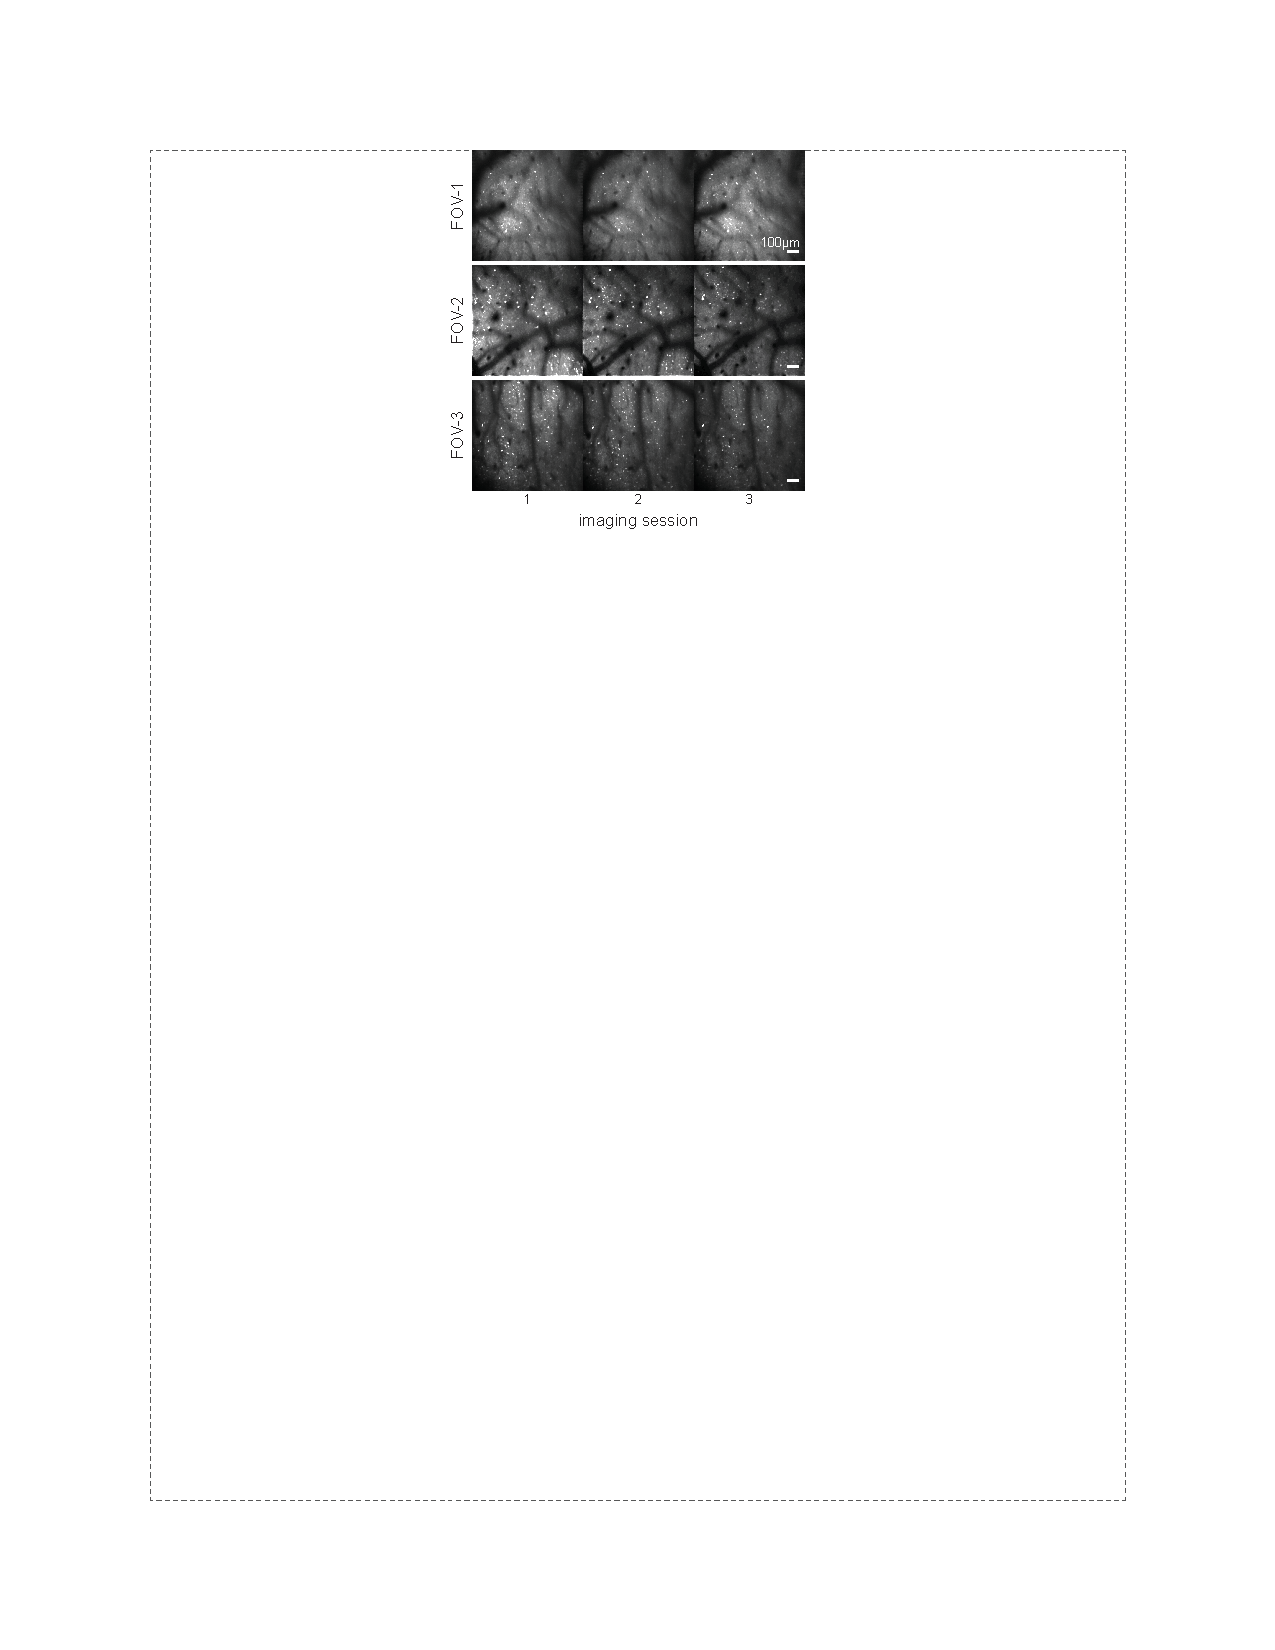
\includegraphics[width=\textwidth]{figures/chapter_2/fig_2-8_multiday_imaging/fig_2-8_multiday_imaging.pdf}
    \vspace{.1in}
    \caption[Multi-day imaging]{Imaging the same cells across days. Each row shows one FOV accessed in three separate days. Each site was identified by eye. Images show the motion-corrected average for each site. No corrections to register one session with the next.    
    \label{fig:multiday_imaging}}
\end{figure}

The kinematic mount for our titanium headplate was not only designed to hold the animal stable, but importantly, to allow precise re-positioning of animals from day to day. In combination with blood vessel landmarks and the unique layout of fluorescent, GCaMP-expressing cell bodies in a given field-of-view in 3-dimensional space, this precise re-fixation allowed us to rapidly relocate the same cells across sessions (Figure\ref{fig:multiday_imaging}). It is difficult in any GCaMP-labeled brain to get the same exact population on each day, due to differences in baseline activity and generic neural tissue movement that occurs across hours. However, the majority of well-labeled cells combined with scanning in depth enabled good matching across sessions. 

% Habituation + shaping
To reduce prohibitively large motion artefacts from rats resisting head-fixation, we developed a shaping procedure to habituate rats for multi-hour sessions (the longest sessions were ~5 hours). Briefly, rats were placed in a red, transparent cylinder also used as enrichment in their home cages, and over the course of several days ($\sim$2-4 days) animals were given decreasing doses of sedative (Midazolam, REFREF mg/kg) and increasingly long habituation sessions (gradually increasing from $\sim$30 minutes to $\sim$3 hours). We found that rats always struggled in the first habituation session without any sedative, which appeared to be critical to accustom the rats to head-fixation in long sessions. That is, most rats quickly learned that it was not possible to physically remove themselves from the implant. We found even in the first two-photon imaging sessions, rats struggled at the very start, well before acquisition began, and remained quiescent throughout most of the session. Although we did not train animals on a task, observable signs indicated that the animals were relatively calm --- they groomed periodically throughout the session, and accepted water and ate treats while they were head-fixed. 

%%%%%%%%%%%%%%%%%%%%%%%
% Concluding remarks
\section{Concluding remarks}
The methodological developments presented in this chapter provide a reliable series of steps for long-term imaging of cranial windows in awake rats. Many of these methods are readily available in mice, and the past decade of systems neuroscience research has seen the surprising emergence of mice as a powerful model system for studying visual circuits. However, the rat has been an important model across all fields of biology for much longer, from sensory behavior\cite{Lashley1930, REFREF} to spatial navigation\cite{REFREF}, to physiological disorders and drug testing\cite{REFREF}. 

We overcome several challenges that have prevented the use of a subset of immensely powerful tools in rat models. First, we developed methods for stably holding an animal by its head, while leaving the rest of its body free to either sit relatively naturally or engage with manipulanda relevant for a behavior task. Second, we fine-tuned standard surgical protocols for cranial window implants that would allow long-term viability for cellular resolution imaging in awake rats. 

Importantly, we demonstrate a method for accessing some of the most lateral and posterior areas of rat cortex. The combination of hard-to-access imaging planes and the rat's capacity for producing large (and damaging) mechanical forces extremely presented significant challenges. Our custom designs for tiling imaging systems overcome these challenges by rotating the optical axis around the animal, allowing a relatively natural sitting position, which is important both for keeping the animal calm during imaging as well as comfortable enough to willingly engage in behaviors. 

We engineered a two-photon microscope design that allows a full repertoire of imaging modes, including multi-channel acquisition and large fields of view that can allow multiple areas to be imaged simultaneously in the rat. These developments unlock significant avenues of research in rats, particularly in questions involving complex behavior and the various functions of different cortical areas, and the nature of their dynamics during learning or particular behaviorally-relevant contexts. 

%%%%%%%%%%%%%%%%%%%%%%%
% While previous studies have shown used coarse retinotopy to identify the areas in which they were recording, the fine-scale retinotopic organization of cell bodies in any extrastriate area remains unknown. To characterize retinotopic preferences at single-cell resolution, we used the same phase-encoding Fourier paradigm used in wide-field mapping with two-photon calcium imaging.


% % Retino scatter
% Cell bodies exhibited a coarse-scale retinotopic organization. However, retinotopic preferences of neighboring cells were disordered and deviated from the surrounding neuropil in V1, LM and LI {\fig:Figure1f, REFREF, Supplemental 2.2, 2.3, stats REFREF}, consistent with findings in mouse visual cortex \cite{Liang2018, Andermann2011, Marques2018}. Single sweeps of the stimulus evoked robust responses in individual cells. 


% We found an asymmetric expansion of spatial representation along the elevation axis in all areas tested (Figure\ref{fig:2p_retino}). There was a ~2-fold increase in cortical magnification along the visual axis of elevation versus azimuth (REFREF paired t-test, V1: p=#, LmL p=#, Li: p=#). 